\chapter{Introducción}
\label{cap:capitulo1}
\setcounter{page}{1}
\pagestyle{plain}

La tarea Sigue-Personas es una de las más empleadas y solicitadas en los Robots de Servicio para multitud de sectores que incorporan soluciones robóticas. El siguiente TFG propone desarrollar dos nuevos ejercicios para la plataforma Unibotics con el objetivo de que los usuarios programen un robot Turtlebot2 tanto en simulado como en real para que realice dicha tarea.\\

Este primer capítulo trata de presentar el estado actual de varios campos de la Robótica que están directamente relacionados con este proyecto para poner en contexto al lector y facilitar su lectura.\\

Por un lado presentaremos la Robótica Móvil, un sector de la robótica que está en constante crecimiento y muy presente en la Robótica de Servicio; por otra parte, introduciremos las Redes Neuronales, un avance significativo en IA que ha permitido realizar aplicaciones muy robustas basadas en la percepción y el razonamiento; y por último hablaremos de la Robótica Educativa, e introduciremos varias plataformas como TheConstruct, Robotics Academy, o Unibotics siendo estas dos últimas las que incorporarán el ejercicio educativo Sigue-Persona.



\section{Robótica Móvil}
\label{sec:robotica_movil}

La robótica es la ciencia que engloba varias ramas tecnológicas o disciplinas, con el objetivo de diseñar máquinas (``robots'') que sean capaces de realizar tareas automatizadas o de simular el comportamiento humano o animal, en función de la capacidad de su software. \cite{revistaderobots}. Su término se remonta a la obra de ciencia ficción escrita por Isaac Asimov: Yo, Robot. (1950)\\

Una vez que la robótica emerge a partir de mediados del siglo XX, surgen 2 sectores: la Robótica Industrial y la Robótica de Servicio. Los \textbf{Robots industriales} se encargan de realizar tareas automatizadas y muy repetitivas en entornos industriales, donde el entorno es controlado. Los \textbf{Robots de Servicio} son aquellos que realizan tareas útiles para el ser humano proporcionándole un servicio. Destacan los robots móviles que permiten desplazarse de un sitio a otro, sin embargo el entorno en el que se enfrentan es bastante heterogéneo, por tanto su software tiene que ser muy robusto para adaptarse correctamente a los cambios.\\

Un \textbf{robot móvil} un sistema electromecánico capaz de desplazarse de ma­nera autónoma sin estar sujeto físicamente a un solo punto. Posee sensores que permiten monitorear a cada momento su posición relativa a su punto de origen (odometría) y a su punto de destino. Normalmente su control es en lazo cerrado. Se clasifican en robots móviles de \textbf{locomoción con ruedas}, \textbf{locomoción con patas} y \textbf{locomoción con orugas}.  Los primeros son más fáciles de controlar pero no se adaptan bien a muchas superficies, sin embargo los robots con patas (cuadrúpedos o bípedos) se adaptan muy bien a distintas superficies pero requieren varios controladores para mantener su equilibrio tanto estático como dinámico.




\subsection{Evolución Histórica}
\label{subsec:evolucion_historica}

Podemos destacar varios hechos importantes a lo largo del siglo XX y principios del XXI que 
marcaron grandes avances en la robótica:

\begin {itemize}
	\item En 1952 aparece la primera máquina de control numérico del MIT que era capaz de automatizar algunas tareas industriales.
	\item En 1961, la compañía Unimates introdujo el primer robot industral en la General Motors.
	\item En 1966, comenzó el desarrollo del primer robot móvil llamado Shakey [Nilsson, 1984]. \ref{fig:shakey}
	\item En los años 70, NASA desarrolló MARS-ROVER, una plataforma móvil que integraba un brazo mecánico, sensores de proximidad, un dispositivo telemétrico láser y cámaras estéreo
	\item En 1997, la NASA envió a Marte un dispositivo móvil llamado Sojourner Rover, para enviar fotografías a la Tierra del planeta rojo. Además, la empresa HONDA sacó el primer humanoide capaz de imitar comportamientos humanos
	\item En 2000, Honda presenta el robot Asimo.
	\item En 2004, Qrio de Sony, un pequeño robot humanoide capaz de correr, bailar, y reconocer caras.
	\item En 2008, SoftBank Robotics presenta el Robot Nao, un robot bípedo dedicado a interactuar con el ser humano y ser muy amigable
	\item En 2013, Boston Dynamics saca a la luz el robot Atlas, un humanoide con actuadores neumáticos. La empresa lo usa para imitar el comportamiento humano llevándolo a otro nivel haciendo acrobacias o incluso parkour.
	\item En 2014, SoftBank Robotics presenta el robot Pepper, robot con forma humana pero se desplaza con ruedas. Se ha usado sobre todo como robot guía, recepcionista y en exhibiciones, sin embargo, fue abandonado en 2021
	\item En 2020, Boston Dynamics saca a la venta el robot cuadrúpedo que imita el comportamiento de un perro llamado Spot, que se usa en algunas fábricas para transportar materiales o realizar tareas de mantenimiento
\end{itemize}

\begin{figure} [h!]
  \begin{center}
    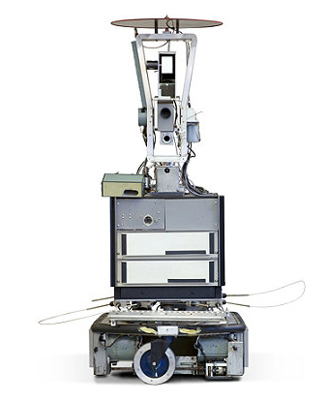
\includegraphics[width=5cm]{imagenes/shakey.jpg}
  \end{center}
  \caption[Shakey (1966-1972)]{Shakey (1966-1972) \cite{shakey-the-robot}.}
  \label{fig:shakey}
\end{figure}\



\subsection{Aplicaciones actuales}
\label{subsec:aplicaciones_actuales}



\section{Redes Neuronales Artificiales (RNA)}
\label{sec:redes_neuronales}

Según \emph{Arthur Samuel}, el Aprendizaje Automático o Machine Learning es el ``campo de estudio que otorga a los ordenadores la capacidad de aprender sin ser programados explícitamente''. Para ello se emplean diversas técnicas dependiendo del objetivo deseado: Regresión Lineal, Regresión Logística, K-NN, K-Means, SVM, Redes Neuronales, Q-Learning, etc.
\\

Cuando incorporamos una RNA, lo que queremos es que nuestro programa o aplicación sepa \textbf{clasificar} unos datos de entrada con su correspondiente salida, habiendo entrenado previamente un modelo computacional inspirado en el cerebro humano. Para ello se le proporciona un set de datos de entrenamiento, donde indicamos, por cada muestra, a qué clase pertenece (Aprendizaje Supervisado). De esta forma, ajustando los valores de unos pesos que se utilizan en el entrenamiento, conseguiremos un nivel de clasificación determinado.\\

Una aplicación de Redes Neuronales es la detección mediante Vision Artificial de objetos. Para ello, se usan modelos de redes de varias capas con un gran número de neuronas (Deep Learning) y de esta forma conseguimos dada una imagen detectar ciertos objetos solicitados como puede ser fruta, coches, utensilios o incluso hasta personas y animales.\\

Típicamente, una Red Neuronal consta de un conjunto de capas formado por varias neuronas que se encuentran interconectadas. Suelen dividirse en 1 capa de entrada, 1 o más capas ocultas y 1 capa de salida. Pero, ¿cómo funciona una neurona?\\

Una neurona, tal y como se muestra en la figura \ref{fig:neurona} está formada pos los siguientes elementos:
\begin{itemize}
	\item \textbf{Valores de Entrada}: Puede ser tanto los valores de las \textbf{características} de cada muestra como la salida de la neurona de una capa anterior.
	\item \textbf{Pesos}: Son unos valores que se optienen al final de la etapa de entrenamiento.
	\item \textbf{Sumatorio}: Esta formado por los productos de los Valores de Entrada por sus correspondientes Pesos
	\item \textbf{Función de Decisión/Activación}: Es una función matemática que se aplica al sumatorio: Lineal, Escalón, Sigmoide, etc
	\item \textbf{Salida}: Es el valor de la función de decisión. Dependiendo de la función de activación usada, la salida será distinta.
\end{itemize}

\begin{figure} [h!]
  \begin{center}
    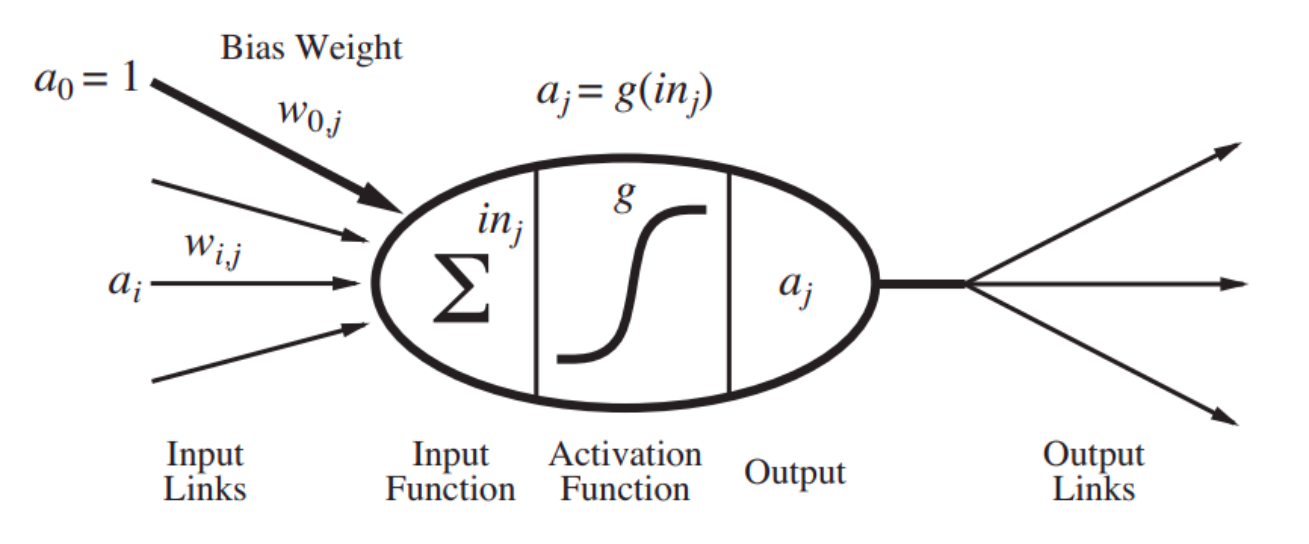
\includegraphics[width=15cm]{imagenes/neurona.png}
  \end{center}
  \caption[Modelo computacional de una neurona]{Modelo computacional de una neurona \cite{AIMA}}
  \label{fig:neurona}
\end{figure}


\subsection{Redes Neuronales Convolucionales (CNN)}
\label{subsec:redes_convolucionales}

\subsection{YOLO}
\label{subsec:yolo}

\subsection{SSD}
\label{subsec:SSD}

\section{Educación en Robótica}
\label{sec:educacion_robotica}

\subsection{Grado en Ingeniería de Robótica Software (URJC, España)}
\label{subsec:grado_robotica_software}
La Universidad Rey Juan Carlos (España) imparte en el campus de Fuenlabrada, el grado en Ingeniería de Robótica Software (primer año: 2018) para enseñar a los futuros ingenieros interesados en este campo a programar la \textbf{inteligencia} de los robots del futuro.\\

Tal y como indica el título del grado, se trata de una carrera universitaria de programación, donde los alumnos abarcarán varios temas como por ejmplo Inteligencia Artificial, visión artificial, programación de lenguajes de alto nivel (C++, Python...), Seguridad, Drones, robots de servicio, robótica industrial, y mucho más. Las clases se imparten tanto en salas de ordenadores con sistemas operativos Linux (distribución Ubuntu) como en el laboratorio de Robótica, donde los alumnos podrán programar directamente robots reales.\\

El robot usado en este Trabajo Fin de Grado es un modelo Turtlebot 2 de Yujin. Consta de una base (kobuki) similar a la de un robot de limpieza con sensores de contaco (bumpers), y un soporte encima que le permite incorporar un RPLIDAR, una cámara, y colocar el portátil del estudiante cuando desarrolla una solución al problema.

\subsection{The Construct}
\label{sec:the_construct}
The Construct es una organización que mantiene una plataforma para aprender robótica con ROS, un framework para programar robots. Imparten varios cursos donde los usuarios acceden a máquinas virtuales con un Linux instalado y todas las dependencias adquiridas. 

\subsection{Robotics Academy}
\label{sec:robotics_academy}
Robotics Academy \cite{robotics-academy} es una colección de ejercicios y desafíos para aprender robótica. Está mantenido por la organización JdeRobot. Sus ejercicios abarcan varios temas: drones, robótica móvil, visión artificial, coches autónomos, robótica industrial, etc. Además es una plataforma Open Source, por lo que cualquier interesado/a puede contribuir desde Github.\\

En sus orígenes, solo se podía ejecutar sobre un sistema operativo Linux, pero desde sus últimas versiones puede ejecutar también sobre Windows y MAC, gracias a la incorporación de plantillas web que se ejecutan en un navegador estableciendo una conexión a través de WebSockets con un contenedor docker que lanza el usuario, permitiendo de esta manera, el despliegue de los ejercicios sobre un sistema operativo virtualizado y con todas sus dependencias ya instaladas.\\

Los usuarios una vez que escogen un ejercicio, lanzan un contenedor docker indicado y automáticamente tienen acceso a una dirección web local donde pueden empezar a programar. La plantilla web incorpora un Editor de Texto y la posibilidad de visualizar un entorno de Gazebo y un terminal mediante una conexión VNC con el contenedor. En la figura \ref{fig:rob-ac-web-template} vemos un ejemplo de plantilla web correspondiente al ejercicio \textit{Follow Person}. La programación se realiza con Python (un lenguaje fácil de entender y aprender, y muy usado en la Robótica).\\

\begin{figure} [h!]
  \begin{center}
    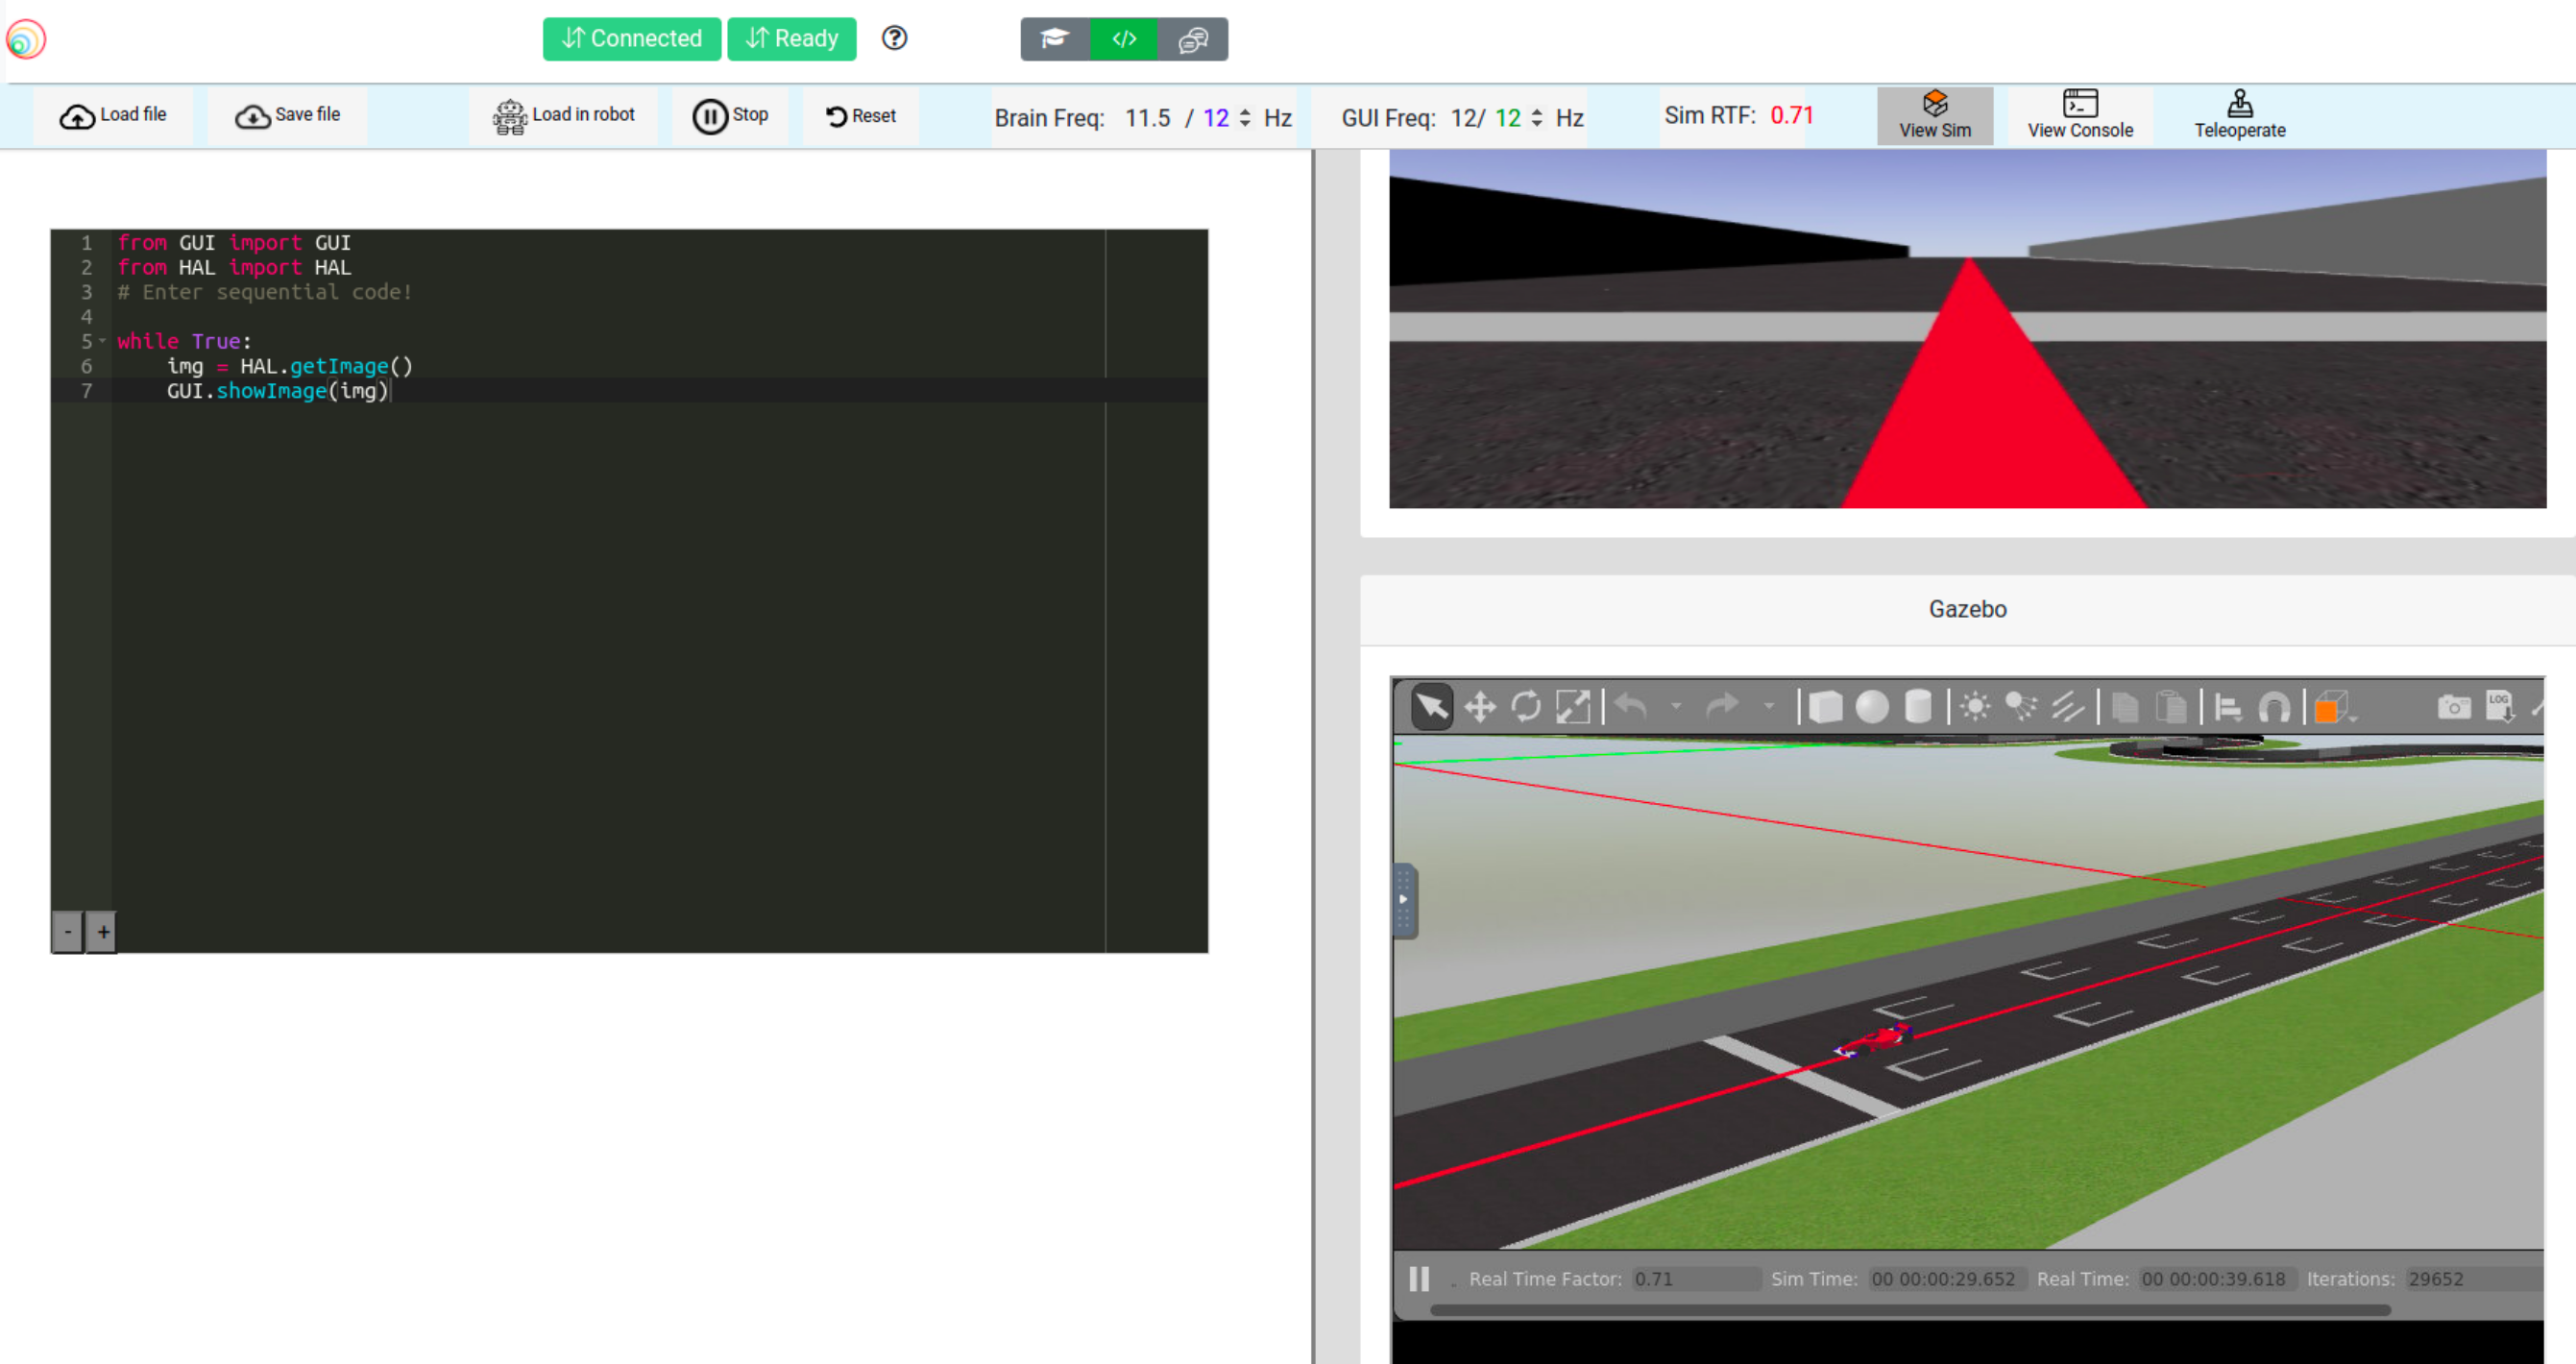
\includegraphics[width=15cm]{imagenes/robotics-academy-web-template.png}
  \end{center}
  \caption[Robotics Academy (Web Template)]{Robotics Academy (Web Template)}
  \label{fig:rob-ac-web-template}
\end{figure}

Una ventaja de usar Robotics Academy, es que permite al usario centrarse única y exclusivamente con el algoritmo que tenga que implementar. Toda la complejidad relacionada con la comunicación con el hardware del robot: motores, laser, cámara, etc. que, por lo general se realiza mediante ROS (un framework para programar Robots) queda encapsulado por 2 módulos: HAL y GUI. De esta manera, el usuario dispone de una API de HAL (Hardware Abstración Layer) para comandar a los actuadores o recibir información de los sensores, y una API de GUI (Graphical User Interface) para visualizar por el navegador información como puede ser una imagen, un mapa o incluso vectores.\\

\subsection{Unibotics}
\label{sec:unibotics}

\textbf{Unibotics} es una plataforma de Robótica que incorpora parte de la coleción de ejercicios de Robotics Academy. Con Unibotics, JdeRobot da un nuevo paso, permitiendo a los usuarios registrarse en un servidor donde pueden guardar sus códigos, acceder cuando deseen, y además, poder contar con la posibilidad de lanzar los ejercicios en un servidor remoto de manera que los usuarios no necesiten instalar docker en sus sistemas operativos.\\

Una vez que el usuario introduce sus credenciales y accede a su sesión, tiene una lista de ejercicios disponibles [Figura \ref{fig:menu-unibotics}], que funcionan de la misma manera que aquellos que proporciona \textit{Robotics Academy}. Actualmente todos los ejercicios disponibles están implementados usando dentro del sistema operativo virtual la distribución ROS Noetic como báse.

Con los 2 nuevos ejercicios Sigue-Personas que explicaremos en este proyecto, pretendemos integrarlos en Unibotics usando ROS Foxy como base. De esta manera, marcaremos un inicio para la migración de varios ejercicios de ROS Noetic a ROS Foxy

\begin{figure} [H]
  \begin{center}
    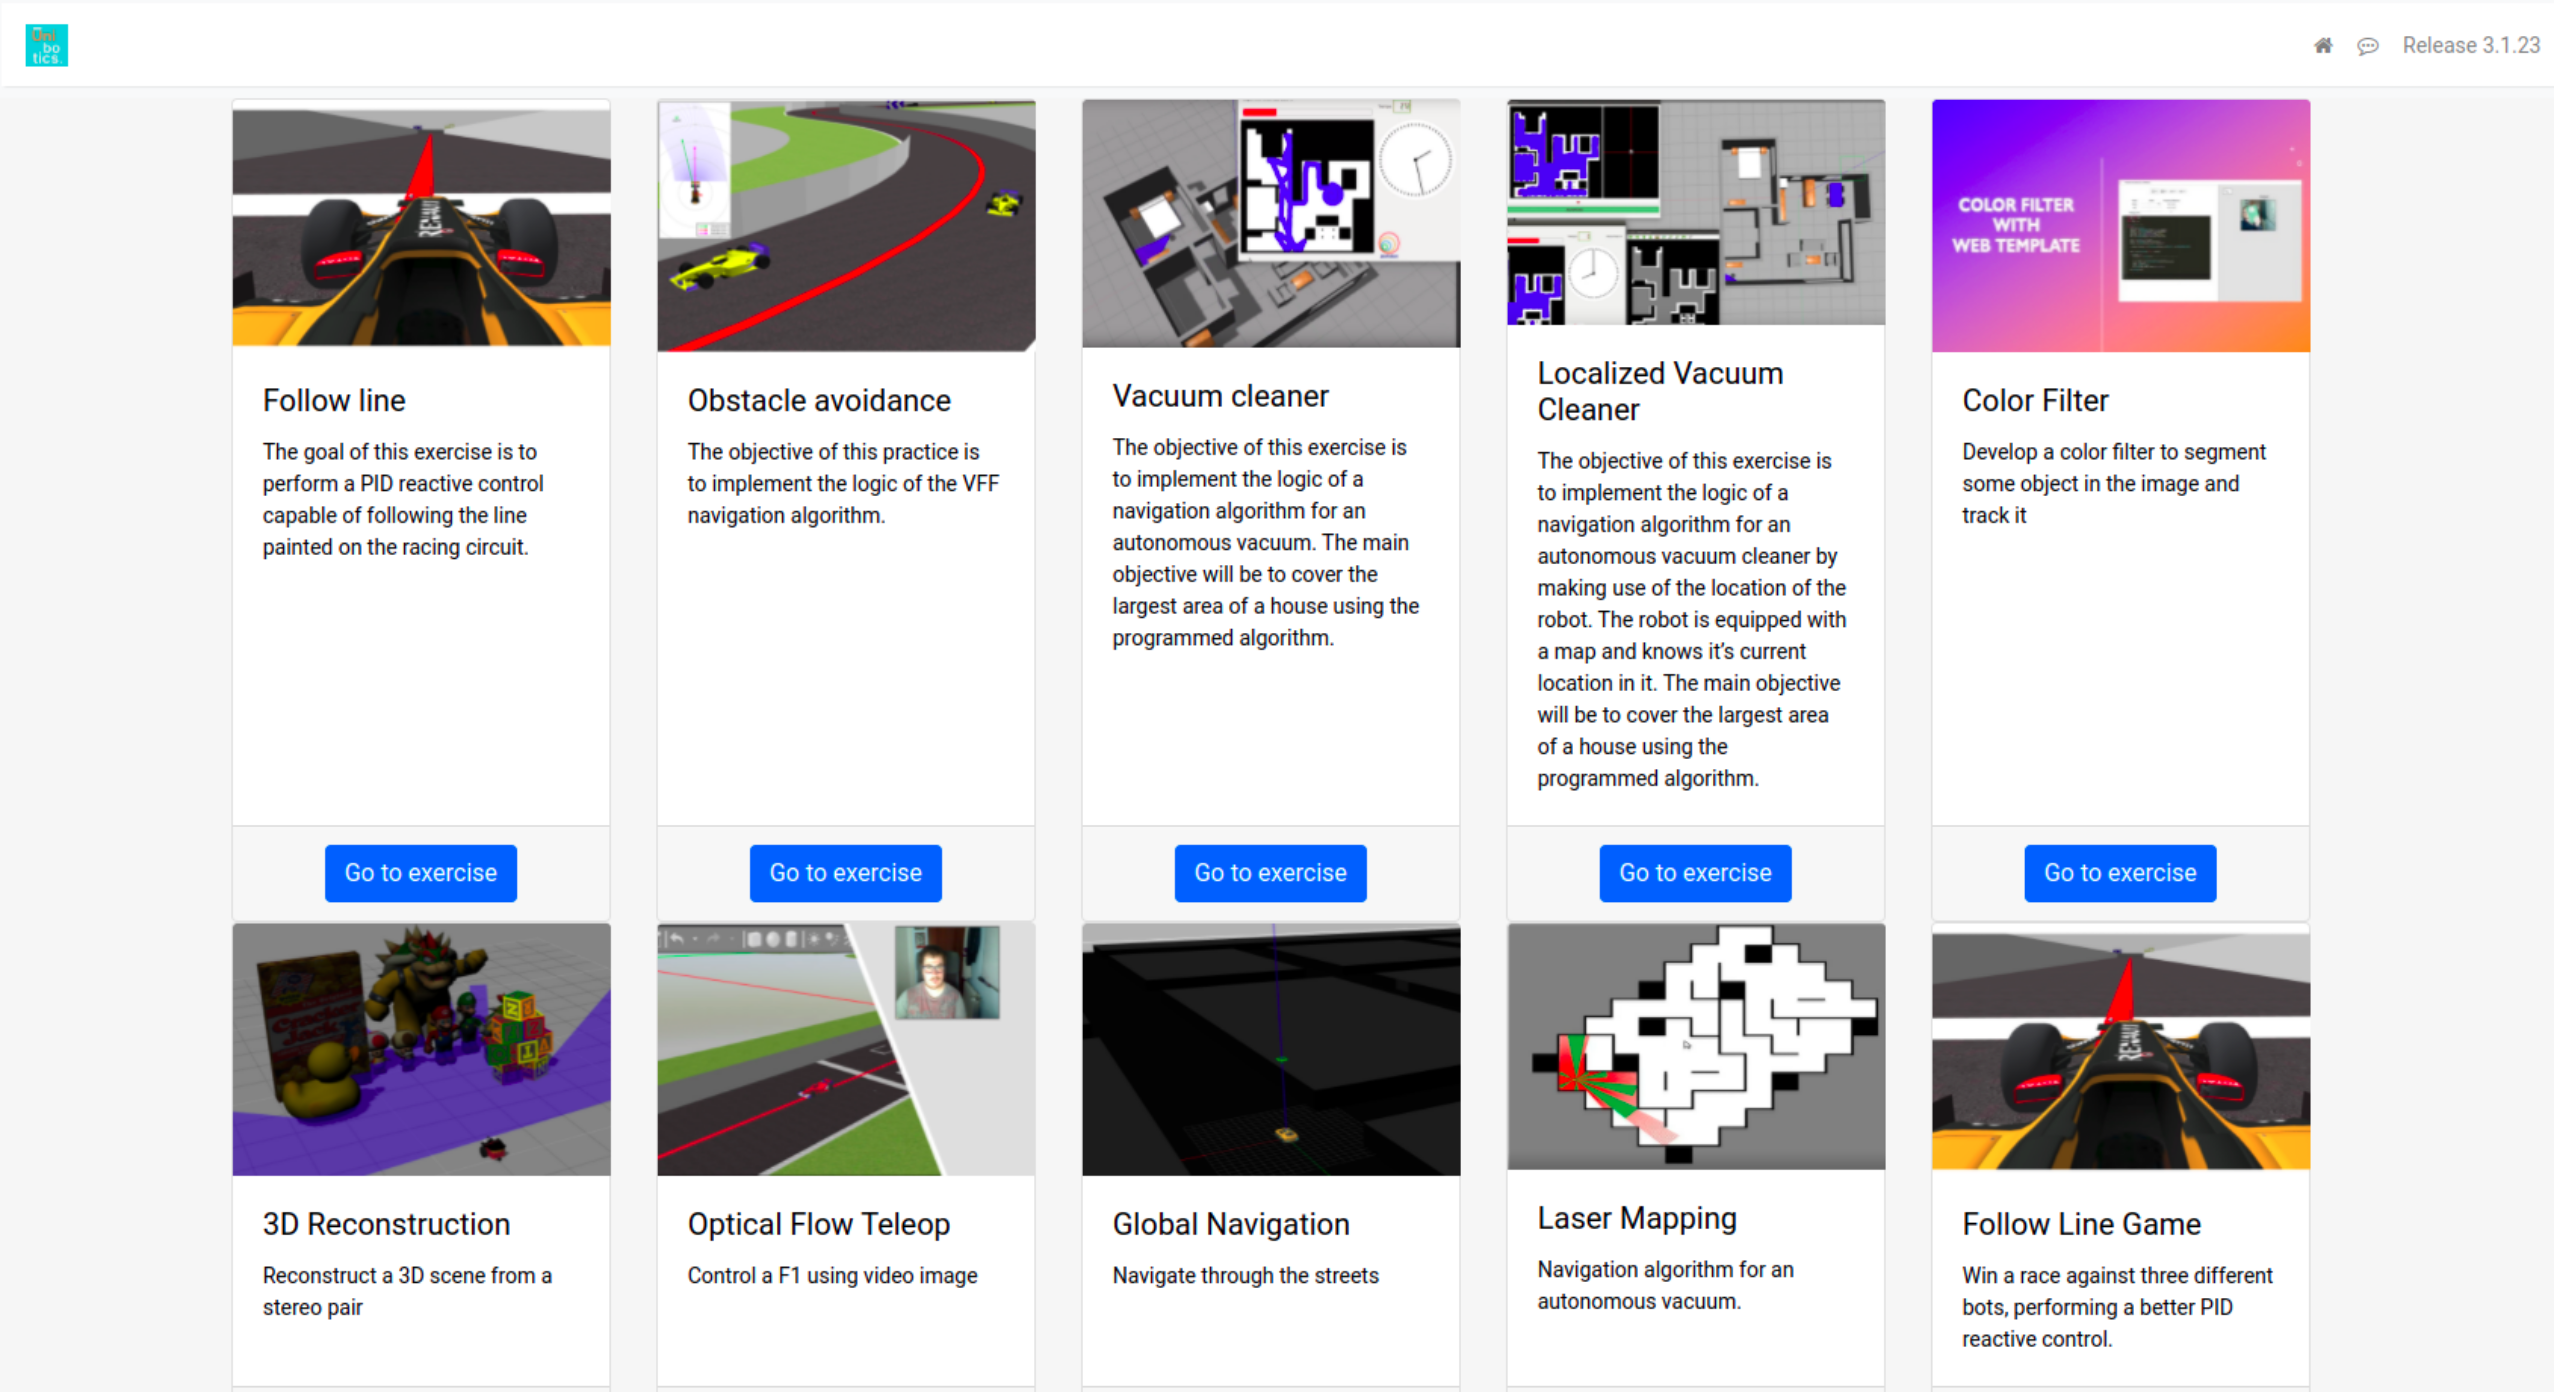
\includegraphics[width=15cm]{imagenes/unibotics-menu.png}
  \end{center}
  \caption[Unibotics (Menú)]{Unibotics (Menú)}
  \label{fig:menu-unibotics}
\end{figure}




